\chapter{Solution Design: Improved Kepler Visualisation Tool}\label{C:sd}

\section{Design features}
\subsection{Visualisation Layout}
\subsubsection{Component Layout}
As the majority of the interaction and movement of visualisation elements occurs in the center of the window it caused a aspect ratio that SOMETHING SOMETHING. It was BETTER to use 2 vertical columns to view and control the visualisation as it had a higher aspect ratio which allowed more of the content to be seen on the screen at once thanks to the fact that the majority of computer screens have a wide ratio.

\begin{figure}[h!]
  \centering
      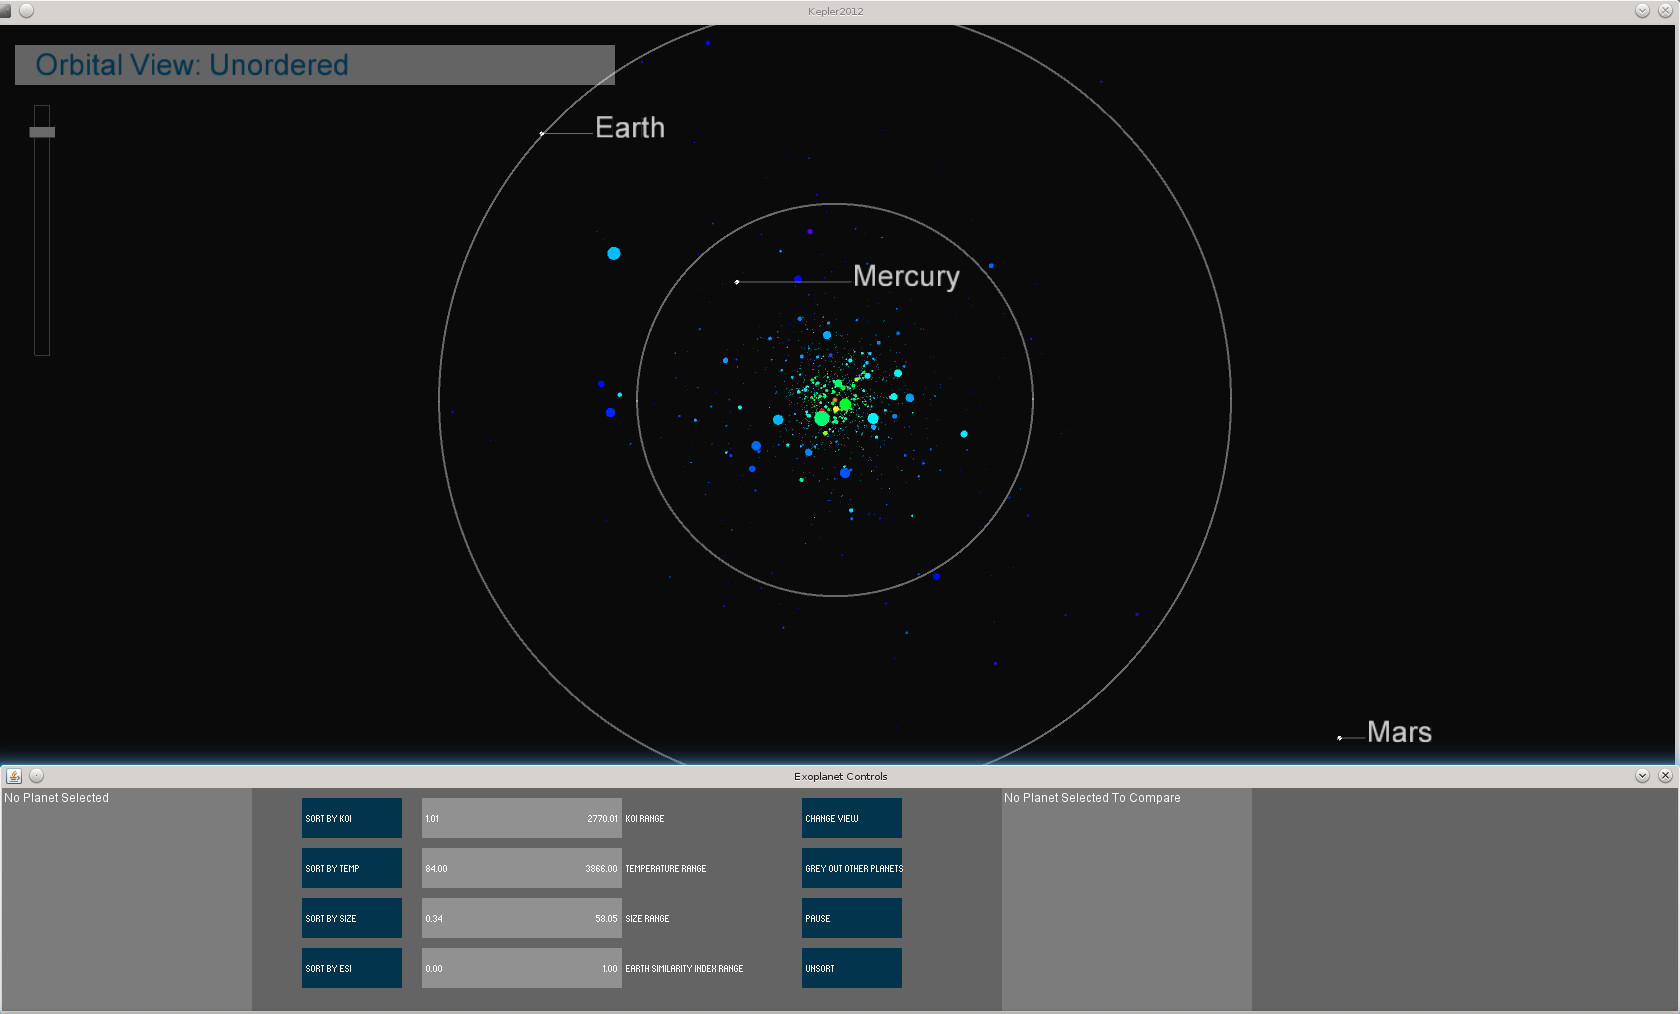
\includegraphics[width=0.8\textwidth]{images/layout_horizontal.jpg}
  \caption{Original Horizontal Layout}  
        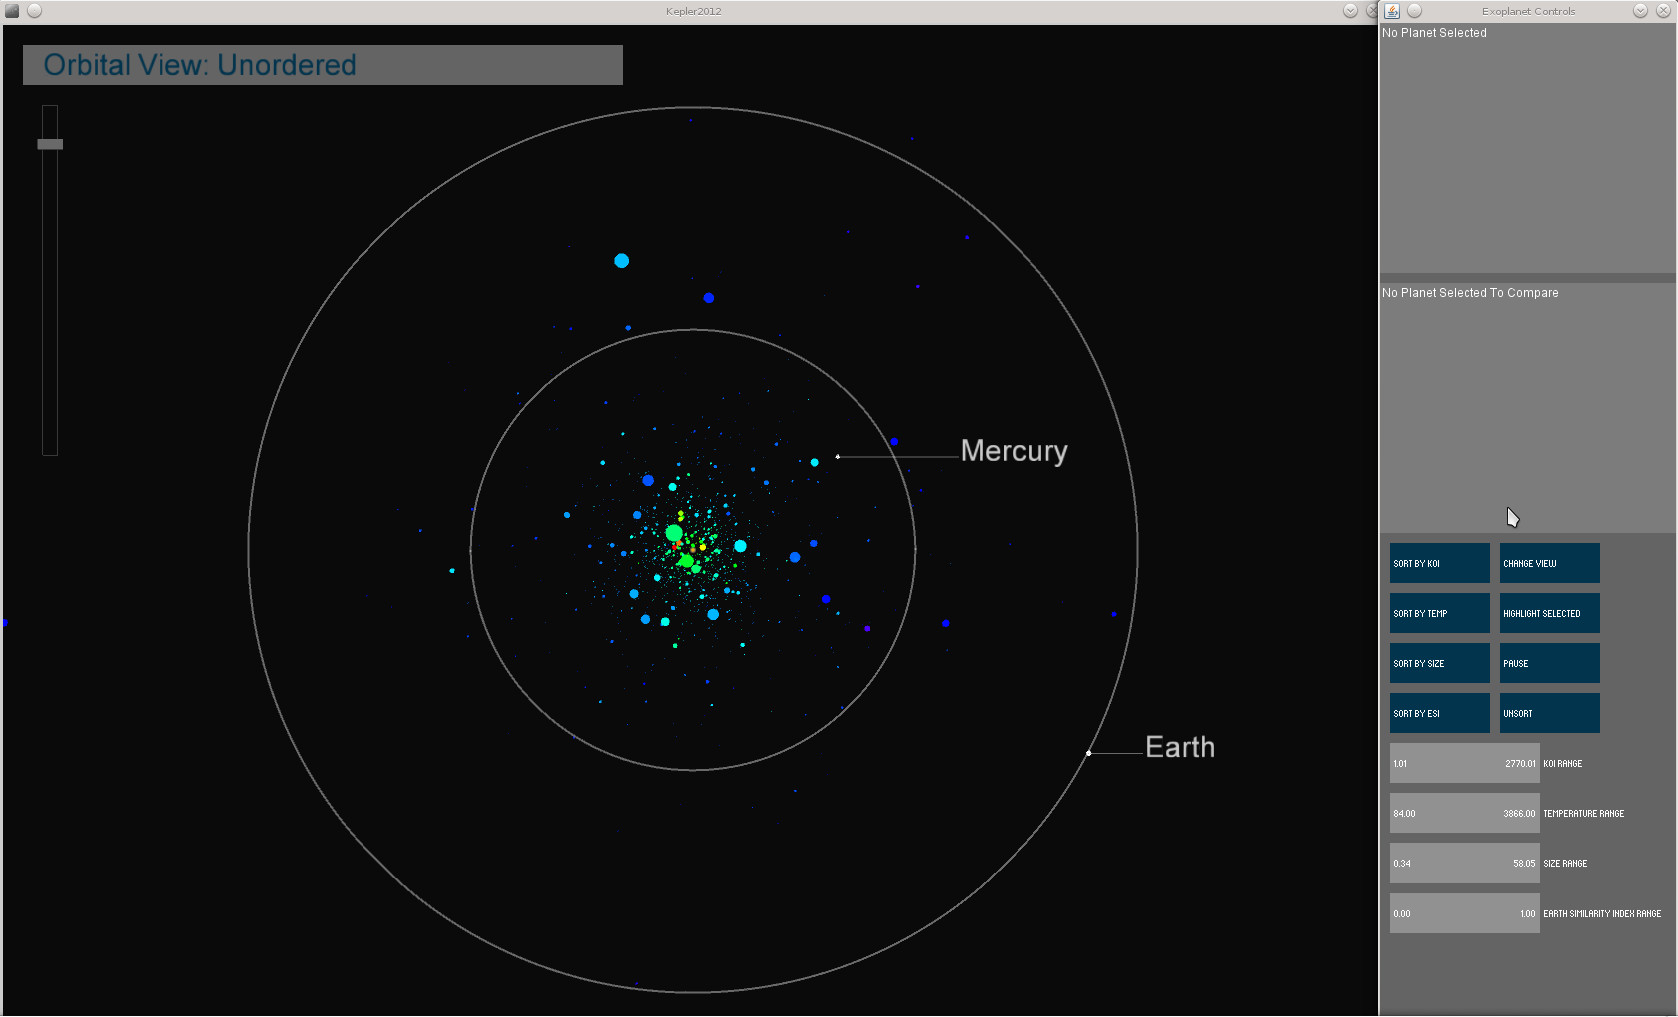
\includegraphics[width=0.8\textwidth]{images/layout_vertical.jpg}
  \caption{Improved Vertical Layout}
\end{figure}

Selection of planets
Kinect for improved user interaction and immersion